\documentclass{amsart}

\usepackage[utf8]{inputenc}
\usepackage[T2A]{fontenc}
\usepackage[english,russian]{babel}
\usepackage{amsthm,amsmath,amsfonts,amssymb}
\usepackage{fullpage}
\usepackage{eufrak}
\usepackage{bbm}

%%% Дополнительная работа с математикой
\usepackage{amsfonts,amssymb,amsthm,mathtools} % AMS
\usepackage{amsmath}
\usepackage{icomma}

%% Шрифты
\usepackage{euscript}	% Шрифт Евклид
\usepackage{mathrsfs}	% Красивый матшрифт

%% Свои команды
\DeclareMathOperator{\lb}{\mathop{lb}}	% логарифм по основанию 2
\DeclareMathOperator{\sgn}{\mathop{sgn}}	% сигнум
\renewcommand{\Im}{\mathop{\mathrm{Im}}\nolimits}	% мнимая часть
\renewcommand{\Re}{\mathop{\mathrm{Re}}\nolimits}	% вещественная часть
\renewcommand{\emptyset}{\varnothing}	% пустое множество
\renewcommand{\le}{\leqslant}	% отечественная версия "меньше или равно"
\renewcommand{\ge}{\geqslant}	% отечественная версия "больше или равно"
\renewcommand{\epsilon}{\varepsilon}	% стандартная "эпсилон"
\renewcommand{\phi}{\varphi}	% стандартная "фи"
\newcommand{\const}{\mathrm{const}}	% константа

%% Множества чисел
\DeclareMathOperator{\Natural}{\mathbb{N}}	% Натуральные числа
\DeclareMathOperator{\Integer}{\mathbb{Z}}	% Целые числа
\DeclareMathOperator{\Integerp}{\mathbb{Z}_{+}}	% Целые неотрицательные числа
\DeclareMathOperator{\Rational}{\mathbb{Q}}	% Рациональные числа
\DeclareMathOperator{\Real}{\mathbb{R}}	% Вещественные числа
\DeclareMathOperator{\Realp}{\mathbb{R}_{>0}}	% Вещественные положительные числа
\DeclareMathOperator{\Realn}{\mathbb{R}_{<0}}	% Вещественные отрицательные числа
\DeclareMathOperator{\Realnn}{\mathbb{R}_{\ge 0}}	% Вещественные неотрицательные числа
\DeclareMathOperator{\Realnp}{\mathbb{R}_{\le 0}}	% Вещественные неположительные числа
\DeclareMathOperator{\Complex}{\mathbb{C}}	% Комплексные числа

%% Заглавные греческие буквы
\DeclareMathOperator{\Alpha}{\mathrm{A}}	% Альфа
\DeclareMathOperator{\Beta}{\mathrm{B}}	% Вета
\DeclareMathOperator{\Epsilon}{\mathrm{E}}	% Эпсилон
\DeclareMathOperator{\Zeta}{\mathrm{Z}}	% Дзета
\DeclareMathOperator{\Eta}{\mathrm{H}}	% Эта
\DeclareMathOperator{\Iota}{\mathrm{I}}	% Йота
\DeclareMathOperator{\Kappa}{\mathrm{K}}	% Каппа
\DeclareMathOperator{\Mu}{\mathrm{M}}	% Мю
\DeclareMathOperator{\Nu}{\mathrm{N}}	% Ню
\DeclareMathOperator{\Omicron}{\mathrm{O}}	% Омикрон
\DeclareMathOperator{\Rho}{\mathrm{P}}	% Ро
\DeclareMathOperator{\Tau}{\mathrm{T}}	% Тау
\DeclareMathOperator{\Chi}{\mathrm{X}}	% Хи

%% Теория вероятностей
\renewcommand{\Prob}{\mathbb P}	% вероятность
\newcommand{\Expect}{\mathbb E}	% математическое ожидание
\renewcommand{\Variance}{\mathbb D}	% дисперсия
\newcommand{\Entropy}{\mathbb H}	% энтропия
\DeclareMathOperator{\cov}{\mathop{cov}}	% ковариация
\DeclareMathOperator{\supp}{\mathop{supp}}	% носитель
\DeclareMathOperator{\Skewness}{\mathop{Skew}}	% коэффициент асимметрии
\DeclareMathOperator{\Kurtosis}{\mathop{Kurt}}	% коэффициент эксцесса

%%% Статистический анализ
\newcommand*{\moment}[1]{\overline{#1}}	% выборочный момент
\DeclareMathOperator{\hskew}{\mathop{\widehat{Skew}}}	% выборочный коэффициент асимметрии
\DeclareMathOperator{\hkurt}{\mathop{\widehat{Kurt}}}	% выборочный коэффициент эксцесса
%% Однопараметрические распределения
\newcommand*{\chisq}[1]{\chi^2_{#1}}	% Распределение хи-квадрат
\newcommand*{\Stud}[1]{\mathcal{S}_{#1}}	% Распределение Стьюдента
\newcommand*{\Exp}[1]{\mathop{\mathrm{Exp}}(#1)}	% Показательное распределение
\newcommand*{\Bern}[1]{\mathop{\mathrm{Bern}}(#1)}	% Распределение Бернулли
\newcommand*{\Geom}[1]{\mathop{\mathrm{Geom}}(#1)}	% Геометрическое распределение
\newcommand*{\Pois}[1]{\mathop{\mathrm{Pois}}(#1)}	% Распределение Пуассона
%% Двухпараметрические распределения
\newcommand*{\FS}[2]{\mathcal{F}_{#1, #2}}	% Распределение Фишера-Снедекора
\newcommand*{\Norm}[2]{\mathcal{N}(#1, #2)}	% Нормальное распределение
\newcommand*{\Unif}[2]{\mathcal{U}(#1, #2)}	% Равномерное распределение
\newcommand*{\DE}[2]{\mathop{\mathrm{DE}}(#1, #2)}	% Распределение Лапласа
\newcommand*{\Cauchy}[2]{\mathop{\mathrm{C}}(#1, #2)}	% Распределение Коши
\newcommand*{\Binom}[2]{\mathop{\mathrm{Binom}}(#1, #2)}	% Биномиальное распределение
\newcommand*{\Betadist}[2]{\mathop{\mathrm{Beta}}(#1, #2)}	% Бета-распределение
\newcommand*{\Gammadist}[2]{\mathop{\mathrm{Gamma}}(#1, #2)}	% Гамма-распределение
%% Ажурные и готические буквы
\newcommand*{\Acl}{\mathcal{A}}	% A красивое
\newcommand*{\Ccl}{\mathcal{C}}	% C красивое
\newcommand*{\Fcl}{\mathcal{F}}	% F красивое
\newcommand*{\Icl}{\mathcal{I}}	% I красивое
\newcommand*{\Kcl}{\mathcal{K}}	% K красивое
\newcommand*{\Pcl}{\mathcal{P}}	% P красивое
\newcommand*{\Ycl}{\mathcal{Y}}	% Y красивое
\newcommand*{\Afr}{\mathfrak{A}}	% A готическое
\newcommand*{\Bfr}{\mathfrak{B}}	% B готическое
\newcommand*{\Ffr}{\mathfrak{F}}	% F готическое
\newcommand*{\Kfr}{\mathfrak{K}}	% K готическое
\newcommand*{\Xfr}{\mathfrak{X}}	% X готическое
%% Теория оценивания
\newcommand*{\ind}[1]{\mathbbm{1}_{\lbrace #1 \rbrace}}	% индикаторная функция
\newcommand*{\bias}[2]{\mathop{\mathrm{bias}}\nolimits_{#1}(#2)}	% смещение

%% Перенос знаков в формулах (по Львовскому)
\newcommand*{\hm}[1]{#1\nobreak\discretionary{}
	{\hbox{$\mathsurround=0pt #1$}}{}}

%%% Работа с картинками
\usepackage{graphicx,xcolor}	% Для вставки рисунков
\graphicspath{{images/}{images2/}}	% папки с картинками
\setlength\fboxsep{3pt}	% Отступ рамки \fbox{} от рисунка
\setlength\fboxrule{1pt}	% Толщина линий рамки \fbox{}
\usepackage{wrapfig}	% Обтекание рисунков и таблиц текстом
\RequirePackage{caption}
\DeclareCaptionLabelSeparator{defffis}{ "--- }
\captionsetup{justification=centering,labelsep=defffis}
\usepackage{float}
\usepackage{tikz}
\usepackage{pgfplots}
\pgfplotsset{compat=newest}
\usetikzlibrary{patterns}
\usetikzlibrary{calc}

%%% Работа с таблицами
\usepackage{array,tabularx,tabulary,booktabs}	% Дополнительная работа с таблицами
\usepackage{longtable}	% Длинные таблицы
\usepackage{multirow}	% Слияние строк в таблице
\usepackage{makecell}
\usepackage{multicol}


\renewcommand{\qedsymbol}{}

\newtheorem{problem}{Задание}

\begin{document}
	\newcommand{\problemset}[1]{
		\begin{center}
			\Large #1
		\end{center}
	}

	\begin{tabbing}
	\hspace{11cm} \= Студент: \= Божко-Домбровский Тимофей \\																			
	\> Группа: \> 2375 \\
	\> Вариант: \> 5 \\	
	\> Дата: \> \today
\end{tabbing}
\hrule
\vspace{1cm}	% файл с заголовком
	\problemset{Теория вероятностей и математическая статистика}
\problemset{Индивидуальное домашнее задание №2}

% Команда ниже задает "название" или слово, которое будет
% отображаться вместо proof или "доказательство"
% поскольку у нас в ИДЗ задачи - то нужно слово "Решение"
\renewcommand*{\proofname}{Решение}

%%%%%%%%%%%%%% ЗАДАНИЕ №1 %%%%%%%%%%%%%%
%% Условие задания №1
\begin{problem}
Распределение случайной величины $\xi $ задано таблицей:
\begin{center}
\begin{table}[h!]
    \centering
    \begin{tabular}{|c|c|c|c|c|c|c|}
        \hline
        $\xi$ & -1 & 0 & 1 & 2 & 3 & $\sum$ \\
        \hline
        $\Prob$ & 1/8 & 1/4 & 1/8 & 1/8 & 3/8 & 1 \\
        \hline
    \end{tabular}
\end{table}
\end{center}
Вычислить $\Expect\xi $, $\Variance\xi $, $\Entropy\xi $ (в натах). Вычислить распределение $ \eta = \cos(\pi\xi/2)$. Построить графики функций распределений $ F_{\xi}(x)$ и $ F_{\eta}(y)$.
\end{problem}

%% Решение задания №1
\begin{proof}
$\supp\xi = \{-1, 0, 1, 2, 3\}$. $\xi$ - дискретная случайная величина (ДСВ). Тогда ее математическое ожидание можно найти по формуле:
\[
\Expect\xi = \sum_{i: p_i > 0} a_i\cdot p_i = -1\cdot\frac{1}{8} + 0\cdot\frac{1}{4} + 1\cdot\frac{1}{8} + 2\cdot\frac{1}{8} + 3\cdot\frac{3}{8} = \frac{11}{8} = 1.375
\]
Для нахождения $\Variance\xi$ воспользуемся свойством: $\Variance\xi = \Expect\xi^2 - (\Expect\xi)^2$; а также формулой для начального момента k-го порядка ДСВ: $\Expect\xi^k = \sum_{i: p_i > 0} a_i^k\cdot p_i$.\\
Тогда:
\begin{gather*}
\Expect\xi^2 = \sum_{i: p_i > 0} a_i^2\cdot p_i = 1\cdot\frac{1}{8} + 0\cdot\frac{1}{4} + 1\cdot\frac{1}{8} + 4\cdot\frac{1}{8} + 9\cdot\frac{3}{8} = \frac{33}{8} = 4\frac{1}{8}\\
\Variance\xi = \Expect\xi^2 - (\Expect\xi)^2 = \frac{33}{8} - \frac{121}{64} = \frac{143}{64} \approx 2.2343
\end{gather*}
Энтропию в натах найдем по известной формуле:
\[
\Entropy\xi = -\sum_{i: p_i > 0} p_i\ln p_i \approx 1.4942 \text{ нат}
\]
$\eta = \cos(\pi\xi/2)$ и $\supp\xi = \{-1, 0, 1, 2, 3\}$.
\begin{gather*}
    \eta(-1) = 0\\
    \eta(0) = 1\\
    \eta(1) = 0\\
    \eta(2) = -1\\
    \eta(3) = 0\\
\end{gather*}
Значит $\supp\eta = \{-1, 0, 1\}$.
\begin{center}
\begin{table}[h!]
    \centering
    \begin{tabular}{|c|c|c|c|c|}
        \hline
        $\eta$ & -1 & 0 & 1 & $\sum$\\
        \hline
        $\Prob$ & 1/8 & 5/8 & 2/8 & 1\\
        \hline
    \end{tabular}
\end{table}
\end{center}
Пояснение к таблице:
\begin{figure}[h!]
    \centering
    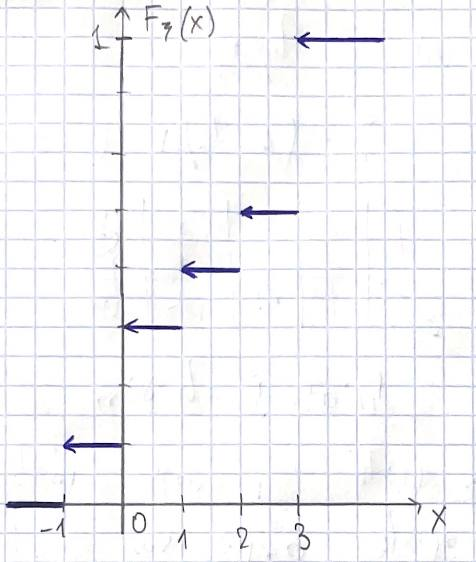
\includegraphics[width=0.5\linewidth]{1.jpg}
    \caption{}
    \label{fig:enter-label}
\end{figure}
\begin{figure}[h!]
    \centering
    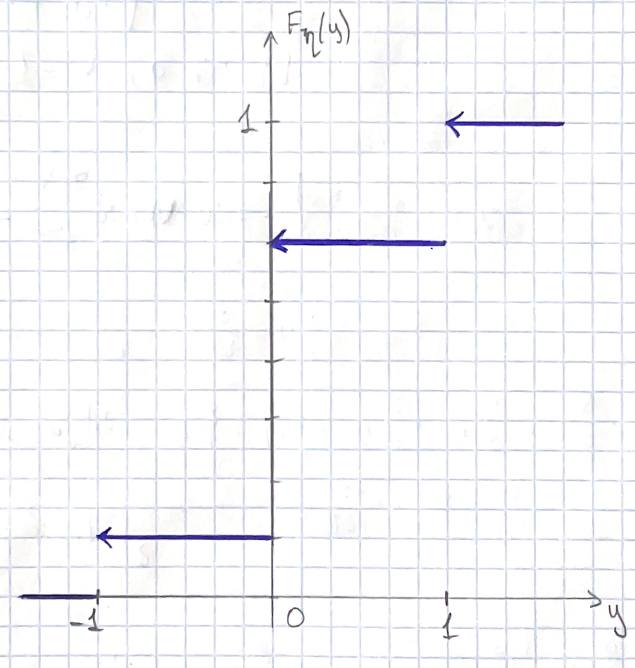
\includegraphics[width=0.5\linewidth]{2.jpg}
    \caption{}
    \label{fig:enter-label}
\end{figure}
\begin{gather*}
    \Prob(\eta = -1) = \Prob(\xi = 2) = \frac{1}{8}\\
    \Prob(\eta = 0) = \Prob(\xi = -1) +  \Prob(\xi = 1) + \Prob(\xi = 3)= \frac{5}{8}\\
    \Prob(\eta = 1) = \Prob(\xi = 0) = \frac{1}{4} = \frac{2}{8}\\
\end{gather*}
Теперь найдем $ F_{\xi}(x)$ и $ F_{\eta}(y)$:
\[ 
F_{\xi}(x) = \begin{cases} 
          0, & x\in (-\infty; -1] \\
          \frac{1}{8}, & x\in (-1; 0] \\
          \frac{3}{8}, & x\in (0; 1] \\
          \frac{4}{8}, & x\in (1; 2] \\
          \frac{5}{8}, & x\in (2; 3] \\
          1, & x\in (3; \infty) \\
       \end{cases}
F_{\eta}(y) = \begin{cases} 
          0, & x\in (-\infty; -1] \\
          \frac{1}{8}, & x\in (-1; 0] \\
          \frac{6}{8}, & x\in (0; 1] \\
          1, & x\in (1; \infty) \\
       \end{cases}
\]
Их графики на рисунках 1 и 2 соответственно.
{\it Ответ:}\\
$\Expect\xi$ = 1.375, $\Variance\xi$ = 2.2343, $\Entropy\xi$ = 1.4942 нат\\

\end{proof}

%%%%%%%%%%%%%% ЗАДАНИЕ №2 %%%%%%%%%%%%%%
%% Условие задания №2
\begin{problem}
Дана плотность распределения абсолютно непрерывной случайной величины $\xi$:
\[ 
p_{\xi}(x) = \begin{cases} 
          C, & x\in [3; 6] \\
          3C, & x\in (6; 8] \\
          0, & \text{в отс. сл.} \\
       \end{cases}
\]
Вычислить С, $\Expect\xi $, $\Variance\xi $, $\Entropy\xi $ (в натах). Вычислить распределение $\eta = \xi^4$. Построить графики функций распределений $ F_{\xi}(x)$ и $ F_{\eta}(y)$.
\end{problem}

%% Решение задания №2
\begin{proof}
Воспользуемся свойством плотности распределения абсолюнто непрерывной случайной величины (АНСВ). Интеграл от плотности по всей числовой прямой должен равняться 1. Тогда:
\[
\int\limits_{-\infty}^{\infty}p_{\xi}(x)dx = C\int\limits_3^6dx + 3C\int\limits_6^8dx = 9C = 1 \Rightarrow C = \frac{1}{9}
\]
И тогда:
\[ 
p_{\xi}(x) = \begin{cases} 
          \frac{1}{9}, & x\in [3; 6] \\
          \frac{1}{3}, & x\in (6; 8] \\
          0, & \text{в отс. сл.} \\
       \end{cases}
\]
Найдем математическое ожидание по известной формуле для АНСВ:
\[
\Expect\xi = \int\limits_{-\infty}^{\infty}x\cdot p_{\xi}(x)dx = \frac{1}{9}\int\limits_3^6xdx + \frac{1}{3}\int\limits_6^8xdx = \frac{27}{18} + \frac{28}{6} = \frac{37}{6} \approx 6.1667
\]
Найдем дисперсию по известному свойству:
\begin{gather*}
\Expect\xi^2 = \int\limits_{-\infty}^{\infty}x^2\cdot p_{\xi}(x)dx = \frac{1}{9}\int\limits_3^6x^2dx + \frac{1}{3}\int\limits_6^8x^2dx = \frac{189}{27} + \frac{296}{9} = \frac{359}{9}\\
\Variance\xi = \Expect\xi^2 - (\Expect\xi)^2 = \frac{359}{9} - \frac{1369}{36} = \frac{67}{36} \approx 1.8611\\
\end{gather*}
Найдем энтропию по известной формуле:
\[
\Entropy\xi = -\int\limits_{-\infty}^{\infty}p_{\xi}(x)\cdot\ln(p_{\xi}(x))dx = -\left(\int\limits_3^6\frac{1}{9}\ln\frac{1}{9}dx + \int\limits_6^8\frac{1}{3}\ln\frac{1}{3}dx\right) \approx 1.4648 \text{нат}
\]
$\supp\xi = [3;8], \eta = \xi^4 \Rightarrow \supp\eta = [81;4096] = [81;1296]\cup[1296;4096]$.\\
1) $\eta\in [81;1296]\Rightarrow\xi\in [3;6]$ и $\eta$ монотонно возрастает.\\
\[
\begin{cases}
    g_1(x) = x^4\\
    g_1^{-1}(y) = \sqrt[4]y\\
\end{cases}
\]
Тогда $p_{1\eta}(y) = \frac{1}{36}\cdot\frac{1}{\sqrt[4]y^3}$.\\
2) $\eta\in [1296; 4096]\Rightarrow\xi\in [6;8]$ и $\eta$ монотонно возрастает.\\
\[
\begin{cases}
    g_2(x) = x^4\\
    g_2^{-1}(y) = \sqrt[4]y\\
\end{cases}
\]
Тогда $p_{2\eta}(y) = \frac{1}{12}\cdot\frac{1}{\sqrt[4]y^3}$.\\
Итого:
\[ 
p_{\eta}(y) = \begin{cases} 
          \frac{1}{36}\cdot\frac{1}{\sqrt[4]y^3}, & y\in [81; 1296] \\
          \frac{1}{12}\cdot\frac{1}{\sqrt[4]y^3}, & x\in (1296; 4096] \\
          0, & \text{в отс. сл.} \\
       \end{cases}
\]
Найдем $ F_{\xi}(x)$ и $ F_{\eta}(y)$:
\begin{figure}[h!]
    \centering
    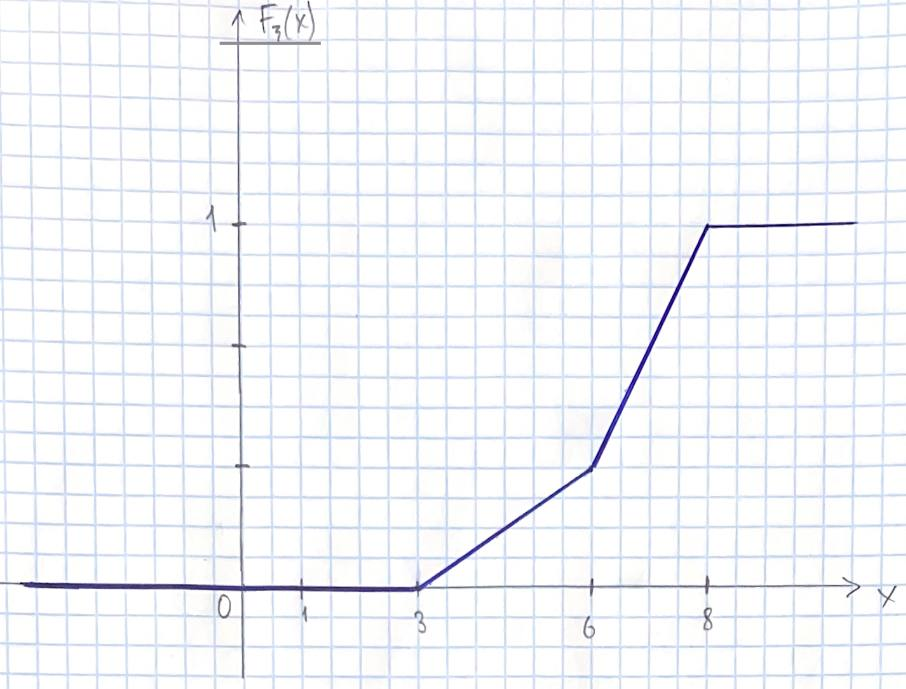
\includegraphics[width=0.5\linewidth]{3.jpg}
    \caption{}
    \label{fig:enter-label}
\end{figure}
\begin{figure}[h!]
    \centering
    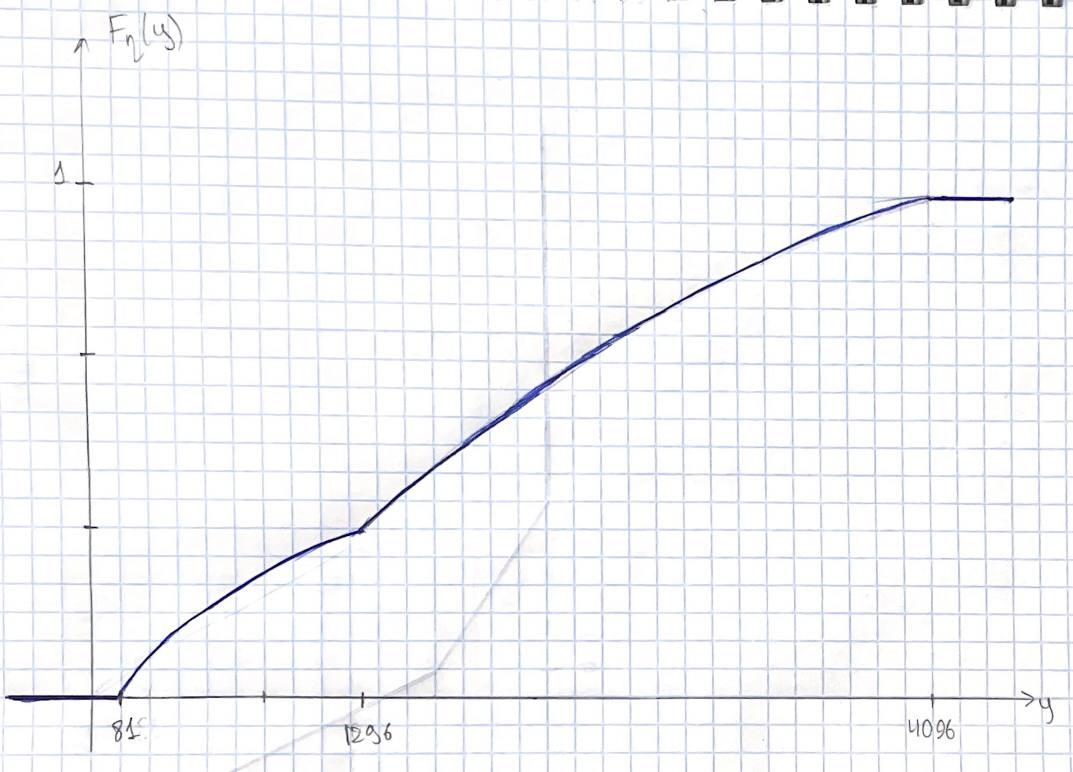
\includegraphics[width=0.5\linewidth]{4.jpg}
    \caption{}
    \label{fig:enter-label}
\end{figure}
\[
F_{\xi}(x) = \int\limits_{-\infty}^xp_{\xi}(t)dt = \begin{cases}
    0, & x\in (-\infty;3]\\
    \frac{x-3}{9}, & x\in (3; 6]\\
    \frac{x-5}{3}, & x\in (6; 8]\\
    1, & x\in (8;\infty)
\end{cases}
\]
\[
F_{\eta}(y) = \int\limits_{-\infty}^yp_{\eta}(t)dt = \begin{cases}
    0, & y\in (-\infty;81]\\
    \frac{\sqrt[4]y-3}{9}, & y\in (81; 1296]\\
    \frac{\sqrt[4]y-5}{3}, & y\in (1296; 4096]\\
    1, & y\in (4096;\infty)
\end{cases}
\]
Их графики на рисунках 3 и 4 соответственно.\\
{\it Ответ:}\\
$\Expect\xi$ = 6.1667, $\Variance\xi$ = 1.8611, $\Entropy\xi$ = 1.4648 нат\\
\end{proof}	% файл с решениями
        %\problemset{Теория вероятностей и математическая статистика}
\problemset{Индивидуальное домашнее задание №0}	% поменяйте номер ИДЗ

\renewcommand*{\proofname}{Решение}

%%%%%%%%%%%%%% ЗАДАНИЕ №1 %%%%%%%%%%%%%%
%% Условие задания №1
\begin{problem}
	Из урны, в которой лежат $ K $ белых и $ L $ чёрных шаров, наудачу выбирают один шар. Чему равна вероятность того, что этот шар "--- белый?
\end{problem}

%% Решение задания №1
\begin{proof}
	Пусть $ A $ "--- событие, что достали белый шар.
	Количество всех исходов будет равно: $ \#\Omega \hm= K + L $.
	
	Тогда количество благоприятных исходов (наступления события $ A $) равно: $ \#A = K $.
	
	Отсюда получаем, что вероятность наступления события $ A $ равна:
	\[ \Prob A = \cfrac{\#A}{\#\Omega} = \cfrac{K}{K + L}. \]
\end{proof}

%%%%%%%%%%%%%% ЗАДАНИЕ №2 %%%%%%%%%%%%%%
%% Условие задания №2
\begin{problem}
	Распределение случайной величины $ \xi $ задано таблицей:
	\begin{center}
		\begin{tabular}{|c|c|c|c|c|c|}
		\hline
		$ \xi $ & 1 & 2 & 4 & 6 & $ \Sigma $ \\
		\hline
		$ \mathbb{P} $ & 0,1 & 0,2 & 0,6 & 0,1 & 1 \\
		\hline
		\end{tabular}
	\end{center}
	Вычислить $ \Expect\xi $, $ \Variance\xi $, $ \Entropy\xi $ (в натах) и распределение $ \eta = \sin(\pi\xi/3) $.
\end{problem}

%% Решение задания №2
\begin{proof}
	Математическое ожидание дискретной случайной величины $ \xi $ задаётся формулой:
	\[ \Expect\xi = \sum_{i \colon p_i > 0}a_ip_i. \]
	Отсюда получаем:
	\[ \Expect\xi = 1 \cdot 0,1 + 2 \cdot 0,2 + 4 \cdot 0,6 + 6 \cdot 0,1 = 3,5. \]
	Дисперсия дискретной случайной величины $ \xi $ задаётся формулой:
	\[ \Variance\xi = \sum_{i \colon p_i > 0}(a_i - \mathbb E\xi)^2p_i. \]
	Отсюда получаем:
	\[ \Variance\xi = (1 - 3,5)^2 \cdot 0,1 + (2 - 3,5)^2 \cdot 0,2 + (4 - 3,5)^2 \cdot 0,6 + (6 - 3,5)^2 \cdot 0,1 = 1,85. \]
	Энтропия дискретной случайной величины $ \xi $ задаётся формулой:
	\[ \Entropy\xi = -\sum_{i \colon p_i > 0}p_i\log_bp_i. \]
	Необходимо вычислить энтропию в натах, т~е. $ b = e $. Получим:
	\[ \Entropy\xi = -(0,1 \cdot \ln0,1 + 0,2 \cdot \ln0,2 + 0,6 \cdot \ln0,6 + 0,1 \cdot \ln0,1) \approx 1,0889. \]
	Носитель случайной величины $ \xi $ имеет вид: $ \supp \xi = \lbrace 1, 2, 4, 6 \rbrace $. Тогда носитель случайной величины $ \eta $ будет иметь вид: $ \supp \eta = \left\lbrace -\frac{\sqrt{3}}{2}, 0, \frac{\sqrt{3}}{2} \right\rbrace  $. Найдём вероятности появления каждого числа:
	\begin{align*}
		\Prob(\eta = -\sqrt{3}/2) &= \Prob(\xi = 4) = 0,6. \\
		\Prob(\eta = 0) &= \Prob(\xi = 6) = 0,1. \\
		\Prob(\eta = \sqrt{3}/2) &= \Prob(\xi = 1) + \Prob(\xi = 2) = 0,3.
	\end{align*}
	Таким образом, можно записать распределение случайной величины $ \eta $ в виде таблицы:
	\begin{center}
		\begin{tabular}{|c|c|c|c|c|}
			\hline
			$ \eta $  & $ -\sqrt{3}/2 $ & 0   & $ \sqrt{3}/2 $ & $ \Sigma $ \\ \hline
			$ \Prob $ & 0,6             & 0,1 & 0,3            & 1          \\ \hline
		\end{tabular}
	\end{center}
\end{proof}

%%%%%%%%%%%%%% ЗАДАНИЕ №3 %%%%%%%%%%%%%%
%% Условие задания №3
\begin{problem}
	Условие задачи №3.
\end{problem}

%% Решение задания №3
\begin{proof}
	Решение задачи №3.
\end{proof}
\end{document}